\begin{questions}


\question{
    The homework repository contains two simple programs that contain bugs. 
    Use valgrind to find these bugs and fix them. Add a short comment to the
    code describing what was wrong and how you fixed the problem. Add the 
    solutions to your repository using the naming convention 
    \texttt{val\_test01\_solved.cpp}, \texttt{val\_test02\_solved.cpp}, and use 
    the Makefile to compile the example problems.
}

\begin{solution}
    Here is a summary of my bug fixes.
    \begin{itemize}
        \item \texttt{val\_test01.cpp}: The code only allocated enough memory for $n$
        Fibonnaci numbers, not $n+1$. It also tried to free its memory with the 
        \texttt{delete} keyword, which only applies to objects created with the
        \texttt{new} keyword.
        \item \texttt{val\_test02.cpp}: The code tries to read uninitialized values
        and write them into other memory addresses. This is unsafe, so I changed the
        code to read only initialized values.
    \end{itemize}
\end{solution}






\question{
  In this homework you will optimize the matrix-matrix multiplication code from 
  the last homework using blocking. This increases the computational intensity 
  (i.e., the ratio of flops per access to the slow memory) and thus speed up 
  the implementation substantially. The code you can start with, along with 
  further instructions are in the source file \texttt{MMult1.cpp}. Specifying what 
  machine you run on, hand in timings for various matrix sizes obtained with the 
  blocked version and the OpenMP version of the code.
}

\begin{solution}
 	I ran this code on a standard CIMS desktop. The processor is an
    Intel(R) Core(TM) i7-8700 CPU @ 3.20GHz. The compiler is \texttt{g++}
    version 4.8.5.
    
    After experimenting with different loop orderings in serial programming,
    I found that the most efficient is to keep the order from \texttt{MMult0.cpp}.
    That is, the outermost loop increments $j=0:n-1$, the middle loop $p=0:k-1$,
    and the inner loop $i=0:m-1$. This is because the matrices are stored on
    the heap in column major order. If we want to access the matrix entries
    sequentially in the order they are stored, then the memory accesses
    \texttt{a[i+p*m]}, \texttt{b[p+j*k]}, and \texttt{c[i+j*m]} require that
    $i$ increments before $p$, $p$ increments before $j$, and that $i$ increments
    before $j$. Thus the loop order we stated is the only one which accesses
    the memory most efficiently. Below, we compare runtimes, flop rate, and 
    bandwidth with another candidate ordering, which we describe next.
    
    Another candidate for efficient ordering comes from minimizing the number of
    reads and writes to memory. We achieve this by incrementing $p$ in the inner
    loop, then $i$, then $j$ in the outer loop so that all operations involving
    the pointer \texttt c can move outside of the innermost loop. We reduce the total
    number of memory accesses, but as we see in Table \ref{tab:MMult1_serial},
    performance decreases since we do not take advantage of the memory structure.
        
    \begin{center}
    \begin{tabular}{|c|c|r|r|r|}
    \hline
    $m=n=k$ & Loop Structure & Runtime (s) & Gflop/s & GB/s \\
    \hline\hline
    256 & $j,p,i$ & 0.003565 &  9.245712 & 111.093007 \\
    \hline
    688 & $j,p,i$ & 0.075147 &  8.751497 & 105.068851 \\
    \hline
    1,024 & $j,p,i$ & 0.316528 &  7.340057 & 88.109357 \\
    \hline
    1,504 & $j,p,i$ & 1.356762 &  5.029314 & 60.365144 \\
    \hline
    1,984 & $j,p,i$ & 3.230298 &  4.854035 & 58.258204 \\
    \hline\hline
    256 & $j,i,p$ & 0.014053 &  1.517237 & 12.185309 \\
    \hline
    688 & $j,i,p$ & 0.298226 &  2.076229 & 16.633973 \\
    \hline
    1,024 & $j,i,p$ & 1.178608 &  1.299286 & 10.404436 \\
    \hline
    1,504 & $j,i,p$ & 6.002820 &  0.966565 &  7.737660 \\
    \hline
    1,984 & $j,i,p$ & 27.613783 &  0.515544 &  4.126432 \\
    \hline
    \end{tabular}
    \captionof{table}{Runtime, flop rate, and bandwidth calculations for serial
        dense matrix multiplication without blocking. All computations use 
        optimization flag \texttt{-O3} and the flag \texttt{-march=native}.}
    \label{tab:MMult1_serial}
    \end{center}
    
    From here on, we assume that matrix multiplication uses the optimal loop ordering
    $j,p,i$. Computational efficiency drops off for $n$ large, beyond about 1,000. We combat
    this by loading blocks of $A$, $B$, and $C$ to the stack. The blocks are sized 
    $K \times K$, with $K \ll n$. Since loading and writing to the blocks does not 
    follow the memory structure of the original existing matrices, we order the code 
    to minimize the number of memory accesses before performing
    the actual matrix multiplication.
    
    After searching for the optimal block size (in multiples of 4) to maximize efficiency,
    we summarize some of our computations in Table \ref{tab:MMult1_block}.
    
    \begin{center}
    \begin{tabular}{|c|c|r|r|r|}
    \hline
    $m=n=k$ & Block size, $K$ & Runtime (s) & Gflop/s & GB/s \\
    \hline\hline
    252 & 12 & 0.004425 &  7.233105 & 99.311679 \\
    \hline
    684 & 12 & 0.090432 &  7.077478 & 96.891084 \\
    \hline
    1,020 & 12 & 0.322679 &  6.577491 & 89.995559 \\
    \hline
    1,500 & 12 & 1.097119 &  6.152478 & 84.149489 \\
    \hline
    1,980 & 12 & 2.531762 &  6.132007 & 83.853641  \\
    \hline\hline
    240 & 120 & 0.002282 & 12.115524 & 148.213250 \\
    \hline
    720 & 120 & 0.062545 & 11.935250 & 145.477435 \\
    \hline
    1,080 & 120 & 0.211550 & 11.909328 & 145.073262 \\
    \hline
    1,560 & 120 & 0.643619 & 11.797092 & 143.652276  \\
    \hline
    1,920 & 120 & 1.207189 & 11.726231 & 142.766863 \\
    \hline\hline
    320 & 160 & 0.005594 & 11.715453 & 142.635645 \\
    \hline
    640 & 160 & 0.045526 & 11.516149 & 139.921211 \\
    \hline
    1,120 & 160 & 0.243995 & 11.516057 & 139.796707 \\
    \hline
    1,600 & 160 & 0.711008 & 11.521672 & 139.815496 \\
    \hline
    1,920 & 160 & 1.235152 & 11.460761 & 139.057231 \\
    \hline
    \end{tabular}
    \captionof{table}{Runtime, flop rate, and bandwidth calculations for serial
        dense matrix multiplication using blocking. All computations use 
        optimization flag \texttt{-O3} and the flag \texttt{-march=native}.}
    \label{tab:MMult1_block}
    \end{center}
    
    The optimal block size appears to be around $K=120$. When the block size is too small,
    about $K < 40$, there is too much overhead cost of forming the blocks and accessing
    memory inefficiently, and the efficiency drops for $n < 1000$. 
    
    We can further improve our performance by parallelizing the matrix-matrix multiplication.
    We perform the parallel version on matrices of size $m=n=k=1920$ with block
    size $K=120$ and compare the runtimes and speedup in Figure \ref{fig:speedup}. We
    can achieve about $55\%$ of the theoretical maximum speedup. However, we are limited
    by the blocking procedure, which is inefficient to parallelize, and the overhead of
    managing multiple threads at once.
    
    \begin{center}
        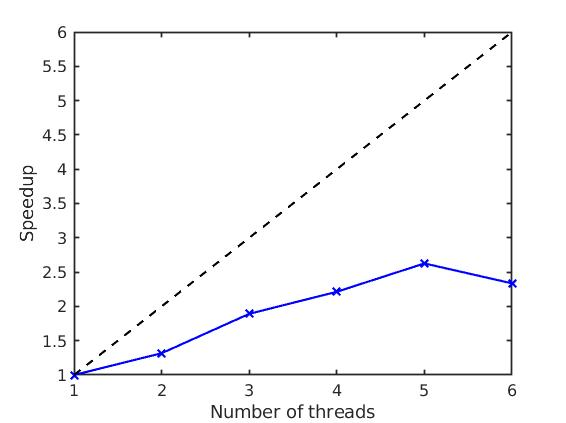
\includegraphics[width=0.7\textwidth]{Images/Matmat_efficiency.jpg}
        \captionof{figure}{Efficiency scaling for our implementation of matrix multiplication}
        \label{fig:speedup}
    \end{center}
    
    
\end{solution}









\question{
  The homework repository contains five OpenMP problems that contain bugs. These 
  files are in C, but they can be compiled with the C++ compiler. Try to find these 
  bugs and fix them. Add a short comment to the code describing what was wrong and
  how you fixed the problem. Add the solutions to your repository using the naming
  convention \texttt{omp\_solved\{2,...\}.c}, and provide a Makefile to compile the 
  fixed example problems.
}

\begin{solution}
    Here is a summary of my bug fixes.
    \begin{itemize}
        \item \texttt{omp\_bug2.c}: I added private variables to the parallel
        region to prevent race conditions. I also restructured the summation 
        operation to prevent a race condition on the variable \texttt{total}.
        I could also have resolved this by adding a reduction statement to 
        the parallel for loop. Finally, the computed sum is large and has many
        terms, so I changed  \texttt{total} from a  \texttt{float} to a 
         \texttt{double} for more precision.
         
        \item \texttt{omp\_bug3.c}: Execution reaches a deadlock since there is a
        \texttt{barrier} directive inside of a function that only two threads access.
        Two possible solutions are to demand only two threads at the beginning
        of the parallel region, or to remove the barrier. I chose the latter, since
        the \texttt{barrier} is unnecessary in the first place.
        
        \item \texttt{omp\_bug4.c}: With $N=1048$, an $N\times N$ array of 
        \texttt{double}s is too large to store on each thread's stack and causes
        a segmentation fault. Possible solutions are to store the array on the heap
        or to increase the thread stack size. I chose the former, since this is a 
        more robust solution. If the code is shared with collaborators, they may
        not be able to support large stack sizes.
        
        \item \texttt{omp\_bug5.c}: It is not clear what the intended purpose of
        this code is. If the code is meant to compute one quantity through two
        different sums and check that the results are equal, then it is impossible
        to accomplish this without radically changing the code structure. On the
        other hand, the main issue at execution is deadlock because of the
        ordering of locks on critical statements. I changed the lock order so that
        one thread ``unlocks B" before the other thread tries to lock it.
        
        \item \texttt{omp\_bug6.c}: The code does not compile because the reduction
        variable in the parallel for loop is private to each thread, when it should
        be shared. I remedy this by creating a shared pointer to a shared variable
        that will store the total sum. Each thread then computes its own dot
        product and adds the result to the shared sum.
    \end{itemize}
\end{solution}







\question{
  Implement first a serial and then an OpenMP version of the two-dimensional Jacobi 
  and Gauss-Seidel smoothers. This is similar to the problem on the first homework 
  assignment, but for the unit square domain $\Omega = (0,1) \cross (0,1)$.
  
  Solve the linear system that arises from a five-point Laplacian stencil applied
  to the Poisson equation
  \[
  \begin{cases}
  -\Delta u = 1 &\text{ on } \Omega \\
  u=0 &\text{ on } \partial\Omega.
  \end{cases}
  \]
  Report timings for different values of $N$ and different numbers of threads. These
  timings should be for a fixed number of iterations, since convergence is slow,
  and slows down even further as $N$ becomes larger.
}

\begin{solution}
    I ran this code on a standard CIMS desktop. The processor is an
    Intel(R) Core(TM) i7-8700 CPU @ 3.20GHz. The compiler is \texttt{g++}
    version 4.8.5. Various run times for my implementations are in Table
    \ref{tab:2DLaplaceRuntime}. We use a relative tolerance of $10^{-6}$
    so that the listed number of iterations does not satisfy the stopping
    criterion on the residual $\norm{Au_k - f}$.

 	\begin{center}
    \begin{tabular}{|c|c|c|c|r|}
    \hline
    $N$ & Iterations & Method & Number of threads & Runtime (s) \\
    \hline\hline
    51 & 3,000 & Jacobi & 1 (serial) & 0.047459 \\ 
    \hline
    51 & 3,000 & Jacobi & 4 & 0.061508 \\ 
    \hline
    51 & 3,000 & Jacobi & 6 & 0.085524 \\ 
    \hline
    51 & 3,000 & Gauss-Seidel & 1 (serial) & 0.017643 \\
    \hline
    51 & 3,000 & Gauss-Seidel & 4 & 0.027840 \\
    \hline
    51 & 3,000 & Gauss-Seidel & 6 & 0.030193 \\
    \hline\hline
    101 & 10,000 & Jacobi & 1 (serial) & 0.684290 \\ 
    \hline
    101 & 10,000 & Jacobi & 4 & 0.406560 \\ 
    \hline
    101 & 10,000 & Jacobi & 6 & 0.409229 \\ 
    \hline
    101 & 10,000 & Gauss-Seidel & 1 (serial) & 0.229584 \\
    \hline
    101 & 10,000 & Gauss-Seidel & 4 & 0.138325 \\
    \hline
    101 & 10,000 & Gauss-Seidel & 6 & 0.131824 \\
    \hline\hline
    1,001 & 10,000 & Jacobi & 1 (serial) & 73.438338 \\ 
    \hline
    1,001 & 10,000 & Jacobi & 4 & 31.234586 \\ 
    \hline
    1,001 & 10,000 & Jacobi & 6 & 34.601011 \\ 
    \hline
    1,001 & 10,000 & Gauss-Seidel & 1 (serial) & 30.342224 \\
    \hline
    1,001 & 10,000 & Gauss-Seidel & 4 & 10.755080 \\
    \hline
    1,001 & 10,000 & Gauss-Seidel & 6 & 11.015953 \\
    \hline
    \end{tabular}
    \captionof{table}{Runtime comparisons for the Jacobi and Gauss-Seidel methods.
    Timings are averages over 100 identical instances of the problem.}
    \label{tab:2DLaplaceRuntime}
    \end{center}
    
    One initially surprising observation is that the Gauss-Seidel method is always
    faster than the Jacobi method for a fixed problem size and thread count, even
    though the update is more complicated for Gauss-Seidel. However, this is
    less surprising when we consider the memory structure for both methods.
    The Gauss-Seidel method only requires \emph{one} copy of the approximate
    solution \texttt u (stored in column major order, \texttt{u[j]} for $0\le 
    j \le N^2-1$), and about half of the memory reads to update \texttt{u[j]} come
    from a spatially local place in memory (\texttt{u[j-1]} and \texttt{u[j+1]}).
    On the other hand, Jacobi requires another copy of the solution from the previous
    iteration, \texttt{u\_old}. Updates always reference \texttt{u\_old}, but 
    \texttt{u\_old} is stored in a completely different memory location from \texttt{u}!
    So, the speedup from spatially local memory accesses is destroyed.
    
    As we expect, for low problem instances ($N<70$), the overhead from parallelization
    causes a slowdown in runtime. Moreover, the overhead of creating and managing six threads
    also causes a slight slowdown compared to the optimal performance of four threads.
    
\end{solution}

\end{questions}